\chapter{Deployment}
\label{cha:deployment}

\section{Github Organization} % (fold)
\label{sec:github}

This project and all its components belong to a Github organization called \texttt{xmlet}\footnote{\href{https://github.com/xmlet}{xmlet Github}}. The aim of that organization is to contain all the related projects to this dissertation. All the generated \ac{DSL}s are also created within this organization. With this approach all the existing projects and future generated \ac{DSL}s can be accessed in one single place.

\section{Maven} % (fold)
\label{sec:maven}

In order to manage the developed projects a tool for project organization and deployment was used, named Maven\footnote{\href{https://maven.apache.org/}{Maven Homepage}}. Maven has the goal of organizing a project in many different ways, such as creating a standard of project building and managing project dependencies. Maven was also used to generate documentation and deploying the projects to a central code repository, Maven Central Repository\footnote{\href{https://search.maven.org/}{Maven Central Repository}}. All the releases of projects belonging to the \texttt{xmlet} Github organization can be found under the same \texttt{groupId}, \href{https://search.maven.org/#search%7Cga%7C1%7Ccom.github.xmlet}{com.github.xmlet}. 

\section{Sonarcloud} % (fold)
\label{sec:sonarcloud}

%TODO Rever e actualizar os dados do SonarCloud.

Code quality and its various implications such as security, low performance and bugs should always be an important issue to a programmer. With that in mind all the projects contained in the \texttt{xmlet} solution were evaluated in various metrics and the results made public for consultation. This way, either future users of those projects or developers trying to improve the projects can check the metrics as another way of validating the quality of the produced code. The tool to perform this evaluation was Sonarcloud\footnote{\href{https://sonarcloud.io/organizations/xmlet/projects}{Sonarcloud xmlet page}}, which provides free of charge evaluations and stores the results which are available for everyone. Sonarcloud also provides an Web \ac{API} to show badges that allow to inform users of different metrics regarding a project. Those badges are presented in the \texttt{xmlet} modules Github pages, as shown in Figure \ref{project_badges} for the XsdParser project.

\begin{figure}[h]
	\centering
	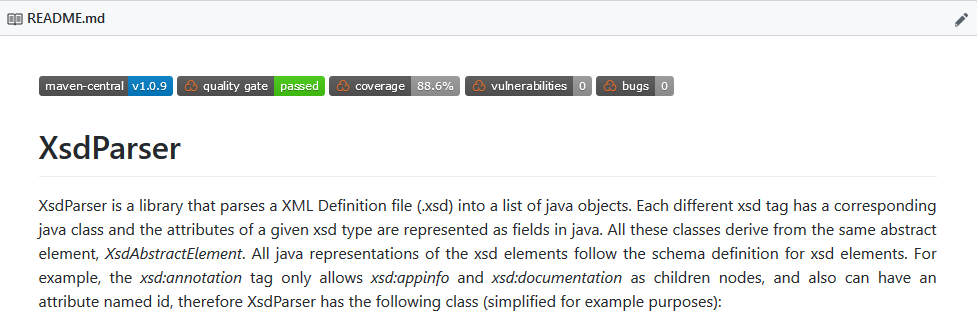
\includegraphics[width=1\textwidth]{badges}
	\caption{XsdParser Github badges}
	\label{project_badges}
\end{figure}

\section{Testing metrics} % (fold)
\label{sec:testingmetrics}

To assert the performance of the \texttt{xmlet} solution we used the \ac{HTML}5 use case to compare it against the multiple solutions. We used all the solutions that were presented in Chapter \ref{cha:stateofart} (J2Html, Rocker, Kotlin). To perform a unbiased comparison instead of creating our own benchmark solution we searched on Github and used two popular benchmarks, this section will contain the results of these benchmarks. The computer used to perform all the tests present in this section has the following specifications:

Processor: Intel Core i3-3217U 1.80GHz\\
RAM: 4GB

\subsection{Spring Benchmark}
\label{sec:springbenchmark}

This was the first benchmark solution we found, which is called \texttt{spring-comparing-template-engines}\footnote{\href{https://github.com/jreijn/spring-comparing-template-engines}{Spring Benchmark}}. This benchmark uses the Spring\footnote{\href{http://spring.io/}{Spring Framework Homepage}} framework to host a web application which serves a route for each template engine to benchmark. Each \textit{template engine} uses the same template and receives the same information to fill the template, which makes it possible to flood all the routes with an high number of requests and assert which route responds faster consequently asserting which \textit{template engine} is faster. This benchmark was promising but was disregarded since it introduced too much \textit{overhead}, e.g. the Spring framework and the additional tool to benchmark the web application, which consumed quite a few resources to perform the requests to the web application. Even though that we didn't end up using this specific benchmark we used the template that it used for the benchmark using another benchmark that added less \textit{overhead}.

\subsection{Template Benchmark}
\label{sec:templatebenchmark}

The second benchmark solution was \texttt{template-benchmark}\footnote{\href{https://github.com/mbosecke/template-benchmark}{Template Benchmark}}. This solution ended up being picked because it introduced less \textit{overhead}. The general idea of the benchmark is the same, it includes many \textit{template engine} solutions which all define the same template and use the same data to generate the complete document. But in this case instead of launching a Spring web application and issuing requests it uses \ac{JMH}\footnote{\href{http://openjdk.java.net/projects/code-tools/jmh/}{Java Microbenchmark Harness}} which is a Java tool to benchmark code. With \ac{JMH} we indicate which methods to benchmark with annotations and configure different benchmark options such as the number of warm-up iterations, the number of measurement iterations or the numbers of threads to run the benchmark method. This benchmark contained eight different \textit{template engines} when we discovered it: Freemarker\cite{freemarker}, Handlebars\cite{handlebars}, Mustache\cite{mustache}, Pebble\cite{pebble}, Thymeleaf\cite{thymeleaf}, Trimou\cite{trimou}, Velocity\cite{velocity} and Rocker\cite{rocker}. These \textit{templates engines}, with the exception of Rocker that we already presented in Chapter \ref{cha:stateofart}, are pretty much classic \textit{template engines}, they all use a text file to define the template, using their own syntax to introduce the dynamic information. In addiction to these we added the solutions presented in the Chapter \ref{cha:stateofart}, J2Html and KotlinX. 

\noindent
The \texttt{template-benchmark} benchmark used only one template, which was the \texttt{Stocks} template. The template is shown in Listing \ref{lst:mustachestockstemplate} using the Mustache idiom.

\bigskip

\lstset{language=HTML, morekeywords={http, equiv}}

\begin{lstlisting}[caption={Stocks Template - Mustache},captionpos=b,label={lst:mustachestockstemplate}]
<!DOCTYPE html>
<html>
	<head>
		<title>Stock Prices</title>
		<meta http-equiv="Content-Type" content="text/html; charset=UTF-8">
		<meta http-equiv="Content-Style-Type" content="text/css">
		<meta http-equiv="Content-Script-Type" content="text/javascript">
		<link rel="shortcut icon" href="/images/favicon.ico">
		<link rel="stylesheet" type="text/css" href="/css/style.css" media="all">
		<script type="text/javascript" src="/js/util.js"></script>
		<style type="text/css">
			<!-- style content -->
		</style>
	</head>
	<body>
		<h1>Stock Prices</h1>
		<table>
			<thead>
	    		<tr>
	     			<th>#</th>
	     			<th>symbol</th>
	     			<th>name</th>
	     			<th>price</th>
	     			<th>change</th>
	     			<th>ratio</th>
	    		</tr>
	   		</thead>
	   		<tbody>
				{{#stockItems}}
	    		<tr class="{{rowClass}}">
	     			<td>{{index}}</td>
	    			<td>
	      				<a href="/stocks/{{value.symbol}}">{{value.symbol}}</a>
	     			</td>
	     			<td>
	      				<a href="{{value.url}}">{{value.name}}</a>
	     			</td>
	     			<td>
	      				<strong>{{value.price}}</strong>
	     			</td>
				     <td{{negativeClass}}>{{value.change}}</td>
				     <td{{negativeClass}}>{{value.ratio}}</td>
	    		</tr>
				{{/stockItems}}
	   		</tbody>
		</table>
	</body>
</html>
\end{lstlisting}

\noindent
This template is pretty straightforward, it describes an \ac{HTML} table which represents information regarding Stock objects, the \texttt{Stock} object is presented in Listing \ref{lst:stock}.

\bigskip

\lstset{language=Java, morekeywords={String}}

\begin{minipage}{\linewidth}
\begin{lstlisting}[caption={Stocks Data Type},captionpos=b,label={lst:stock}]
public class Stock {
    private int index;
    private String name;
    private String url;
    private String symbol;
    private double price;
    private double change;
    private double ratio;    
}
\end{lstlisting}
\end{minipage}

\noindent
Apart from this template and its associated data type that were already present in this benchmark solution we also used another template, the Presentations template, which was featured in the \texttt{spring-comparing-template-engines} solution. The Presentations template is as follow in Listing \ref{lst:mustachepresentationstemplate} and the respective \texttt{Presentation} object in Listing \ref{lst:presentation}.

\bigskip

\lstset{language=HTML, morekeywords={http, equiv}}

\begin{lstlisting}[caption={Stocks Template - Mustache},captionpos=b,label={lst:mustachepresentationstemplate}]
<!DOCTYPE html>
<html>
	<head>
		<meta charset="utf-8">
		<meta name="viewport" content="width=device-width, initial-scale=1.0">
		<meta http-equiv="content-language" content="IE=Edge">
		<title>
			JFall 2013 Presentations - htmlApi
		</title>
		<link rel="Stylesheet" href="/webjars/bootstrap/3.3.7-1/css/bootstrap.min.css" media="screen">
	</head>
	<body>
		<div class="container">
			<div class="page-header">
				<h1>
					JFall 2013 Presentations - htmlApi
				</h1>
			</div>
			{{#presentationItems}}
			<div class="panel panel-default">
				<div class="panel-heading">
					<h3 class="panel-title">
						{{title}} - {{speakerName}}
					</h3>
				</div>
				<div class="panel-body">
					{{summary}}
				</div>
			</div>
			{{/presentationItems}}
		</div>
		<script src="/webjars/jquery/3.1.1/jquery.min.js">
		</script>
		<script src="/webjars/bootstrap/3.3.7-1/js/bootstrap.min.js">
		</script>
	</body>
</html>
\end{lstlisting}

\bigskip

\lstset{language=JAVA, morekeywords={String}}

\begin{minipage}{\linewidth}
\begin{lstlisting}[caption={Presentation Data Type},captionpos=b,label={lst:presentation}]
public class Presentation {
    private String title;
    private String speakerName;
    private String summary;
}
\end{lstlisting}
\end{minipage}

\noindent
By using two different templates the objective was to observe if the results were maintained throughout the different solutions. The main difference between both templates are that the Stocks template introduces much more \textit{placeholders} for two different reasons, it has more fields that will be accessed in the template and has twenty objects in the default data set while Presentations only has ten objects in his data set. This means that the Stocks template will generate more \texttt{String} operations to the classic \textit{template engine} solutions and more Java method calls for the solutions that have the template defined within the Java language.  

\noindent
Now that we have two distinct templates implemented by over ten distinct solutions how will we benchmark these solutions? We have two methods, one for the Stocks template and other Presentations template, in each \textit{template engine} solution that will obtain/generate the template and insert a default set of elements for each template. Both these method are annotated with the \texttt{@Benchmark} annotation. We generate a \ac{JAR} containing all these benchmark methods and will use the command line to perform the benchmark, removing the \ac{IDE} \textit{overhead}. The generated methods will then be benchmarked in two different variants, one with uses a single thread to run the benchmark method and other that uses four threads, the number of cores of the testing machine, to run the benchmark method. The results presented in this section are a result of the mean value of five forked iterations, each one of the forks running eight different iterations, performed after eight warm-up iterations. This approach intends to remove any outlier values from the benchmark. The benchmark values were obtained with the computer without any open programs, background tasks, only with the command line running the benchmark.

\pgfplotsset{compat=1.5}

\begin{figure}[H]
\centering
\captionsetup{justification=centering}
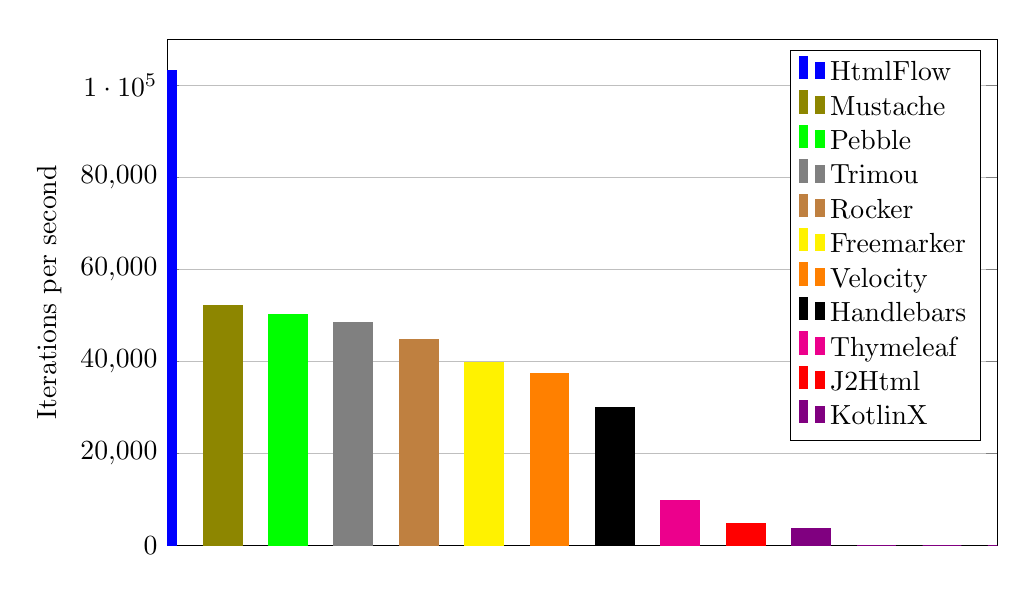
\begin{tikzpicture}
    \begin{axis}[
        width  = 1*\textwidth,
        height = 8cm,
        major x tick style = transparent,
        ybar=1*\pgflinewidth,
        bar width=14pt,
        ymajorgrids = true,
        ylabel = {Iterations per second},
		symbolic x coords={HtmlFlow,Mustache,Pebble,Trimou,Rocker,Freemarker,Velocity,Handlebars,Thymeleaf,J2Html,KotlinX, dummy1, dummy2, dummy3},
        %xtick = data,
        xticklabels = {},
        scaled y ticks = false,
        enlarge x limits=0.75,
        ymin=0,
        ymax=110000,
        legend cell align=left,]
                
        \addplot[style={blue,fill=blue,mark=none}]
            coordinates {(HtmlFlow, 103277)};
        \addplot[style={olive,fill=olive,mark=none}]
            coordinates {(Mustache, 52196)};
        \addplot[style={green,fill=green,mark=none}]
            coordinates {(Pebble, 50218)};
        \addplot[style={gray,fill=gray,mark=none}]
            coordinates {(Trimou, 48548)};
        \addplot[style={brown,fill=brown,mark=none}]
            coordinates {(Rocker, 44718)};
        \addplot[style={yellow,fill=yellow,mark=none}]
            coordinates {(Freemarker, 39711)};
        \addplot[style={orange,fill=orange,mark=none}]
            coordinates {(Velocity, 37409)};
        \addplot[style={black,fill=black,mark=none}]
            coordinates {(Handlebars, 30029)};
        \addplot[style={magenta,fill=magenta,mark=none}]
            coordinates {(Thymeleaf, 9631)};
        \addplot[style={red,fill=red,mark=none}]
            coordinates {(J2Html, 4650)};
        \addplot[style={violet,fill=violet,mark=none}]
            coordinates {(KotlinX, 3661)};
        \addplot[style={violet,fill=violet,mark=none}]
            coordinates {(dummy1, 0)};
        \addplot[style={violet,fill=violet,mark=none}]
            coordinates {(dummy2, 0)};
        \addplot[style={violet,fill=violet,mark=none}]
            coordinates {(dummy3, 0)};
        \legend{HtmlFlow,Mustache,Pebble,Trimou,Rocker,Freemarker,Velocity,Handlebars,Thymeleaf,J2Html,KotlinX}
    \end{axis}
\end{tikzpicture}
\caption{Benchmark Presentations - 1 Thread}
\label{fig:benchpresentations1thread}
\end{figure}

\newpage

\begin{figure}[H]
\centering
\captionsetup{justification=centering}
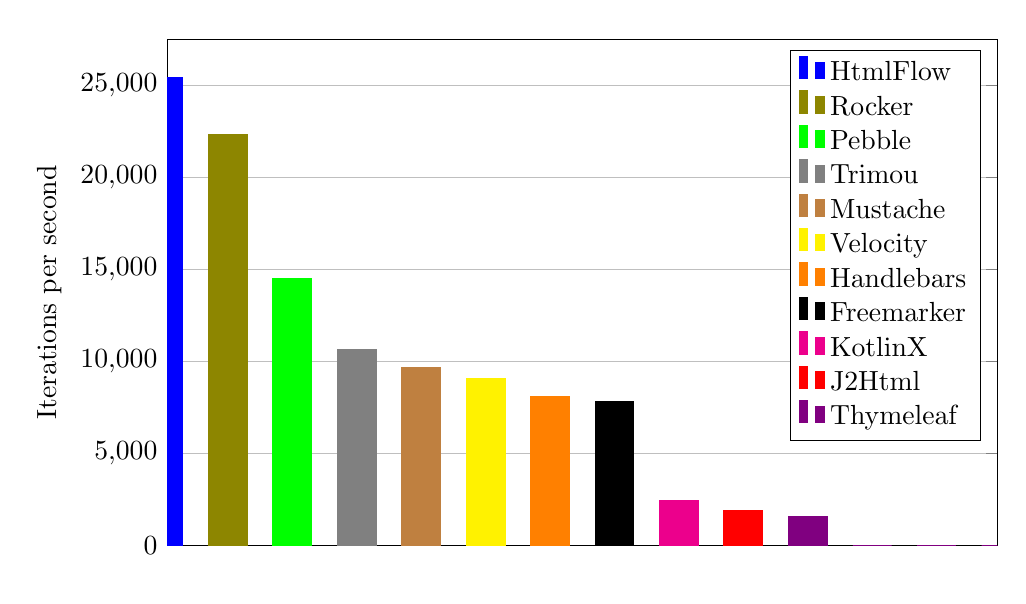
\begin{tikzpicture}
    \begin{axis}[
        width  = 1*\textwidth,
        height = 8cm,
        major x tick style = transparent,
        ybar=1*\pgflinewidth,
        bar width=14pt,
        ymajorgrids = true,
        ylabel = {Iterations per second},
		symbolic x coords={HtmlFlow,Rocker,Pebble,Trimou,Mustache,Velocity,Handlebars,Freemarker,KotlinX,J2Html,Thymeleaf, dummy1, dummy2, dummy3},
        %xtick = data,
        xticklabels = {},
        scaled y ticks = false,
        enlarge x limits=0.8,
        ymin=0,
        ymax=27500,
        legend cell align=left,]
                
        \addplot[style={blue,fill=blue,mark=none}]
            coordinates {(HtmlFlow, 25448)};
        \addplot[style={olive,fill=olive,mark=none}]
            coordinates {(Rocker, 22324)};
        \addplot[style={green,fill=green,mark=none}]
            coordinates {(Pebble, 14494)};
        \addplot[style={gray,fill=gray,mark=none}]
            coordinates {(Trimou, 10666)};
        \addplot[style={brown,fill=brown,mark=none}]
            coordinates {(Mustache, 9643)};
        \addplot[style={yellow,fill=yellow,mark=none}]
            coordinates {(Velocity, 9079)};
        \addplot[style={orange,fill=orange,mark=none}]
            coordinates {(Handlebars, 8093)};
        \addplot[style={black,fill=black,mark=none}]
            coordinates {(Freemarker, 7789)};
        \addplot[style={magenta,fill=magenta,mark=none}]
            coordinates {(KotlinX, 2429)};
        \addplot[style={red,fill=red,mark=none}]
            coordinates {(J2Html, 1870)};
        \addplot[style={violet,fill=violet,mark=none}]
            coordinates {(Thymeleaf, 1560)};
        \addplot[style={violet,fill=violet,mark=none}]
            coordinates {(dummy1, 0)};
        \addplot[style={violet,fill=violet,mark=none}]
            coordinates {(dummy2, 0)};
        \addplot[style={violet,fill=violet,mark=none}]
            coordinates {(dummy3, 0)};
        \legend{HtmlFlow,Rocker,Pebble,Trimou,Mustache,Velocity,Handlebars,Freemarker,KotlinX,J2Html,Thymeleaf}
    \end{axis}
\end{tikzpicture}
\caption{Benchmark Stocks - 1 Thread}
\label{fig:benchstocks1thread}
\end{figure}

\bigskip

\begin{figure}[H]
\centering
\captionsetup{justification=centering}
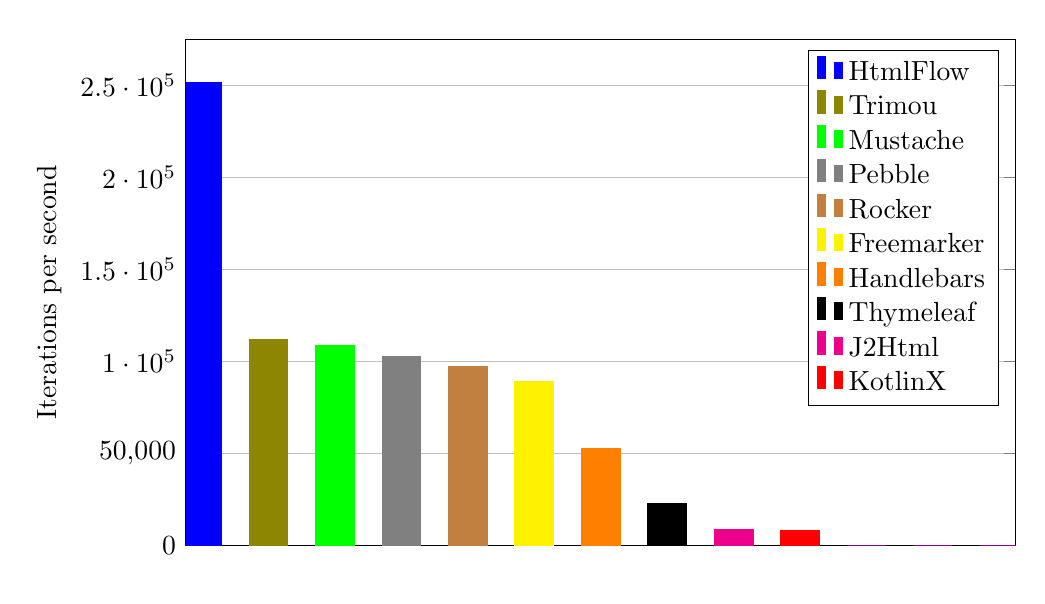
\begin{tikzpicture}
    \begin{axis}[
        width  = 1*\textwidth,
        height = 8cm,
        major x tick style = transparent,
        ybar=1*\pgflinewidth,
        bar width=14pt,
        ymajorgrids = true,
        ylabel = {Iterations per second},
		symbolic x coords={HtmlFlow,Trimou,Mustache,Pebble,Rocker,Freemarker,Handlebars,Thymeleaf,J2Html,KotlinX, dummy1, dummy2, dummy3},
        %xtick = data,
        xticklabels = {},
        scaled y ticks = false,
        enlarge x limits=0.8,
        ymin=0,
        ymax=275000,
        legend cell align=left,]
                
        \addplot[style={blue,fill=blue,mark=none}]
            coordinates {(HtmlFlow, 251521)};
        \addplot[style={olive,fill=olive,mark=none}]
            coordinates {(Trimou, 111806)};
        \addplot[style={green,fill=green,mark=none}]
            coordinates {(Mustache, 108431)};
        \addplot[style={gray,fill=gray,mark=none}]
            coordinates {(Pebble, 102791)};
        \addplot[style={brown,fill=brown,mark=none}]
            coordinates {(Rocker, 97296)};
        \addplot[style={yellow,fill=yellow,mark=none}]
            coordinates {(Freemarker, 88909)};
        \addplot[style={orange,fill=orange,mark=none}]
            coordinates {(Handlebars, 52626)};
        \addplot[style={black,fill=black,mark=none}]
            coordinates {(Thymeleaf, 22889)};
        \addplot[style={magenta,fill=magenta,mark=none}]
            coordinates {(J2Html, 8513)};
        \addplot[style={red,fill=red,mark=none}]
            coordinates {(KotlinX, 7998)};
        \addplot[style={violet,fill=violet,mark=none}]
            coordinates {(dummy1, 0)};
        \addplot[style={violet,fill=violet,mark=none}]
            coordinates {(dummy2, 0)};
        \addplot[style={violet,fill=violet,mark=none}]
            coordinates {(dummy3, 0)};
        \legend{HtmlFlow,Trimou,Mustache,Pebble,Rocker,Freemarker,Handlebars,Thymeleaf,J2Html,KotlinX}
    \end{axis}
\end{tikzpicture}
\caption{Benchmark Presentations - 4 Threads}
\label{fig:benchpresentations4threads}
\end{figure}

\newpage

\begin{figure}[H]
\centering
\captionsetup{justification=centering}
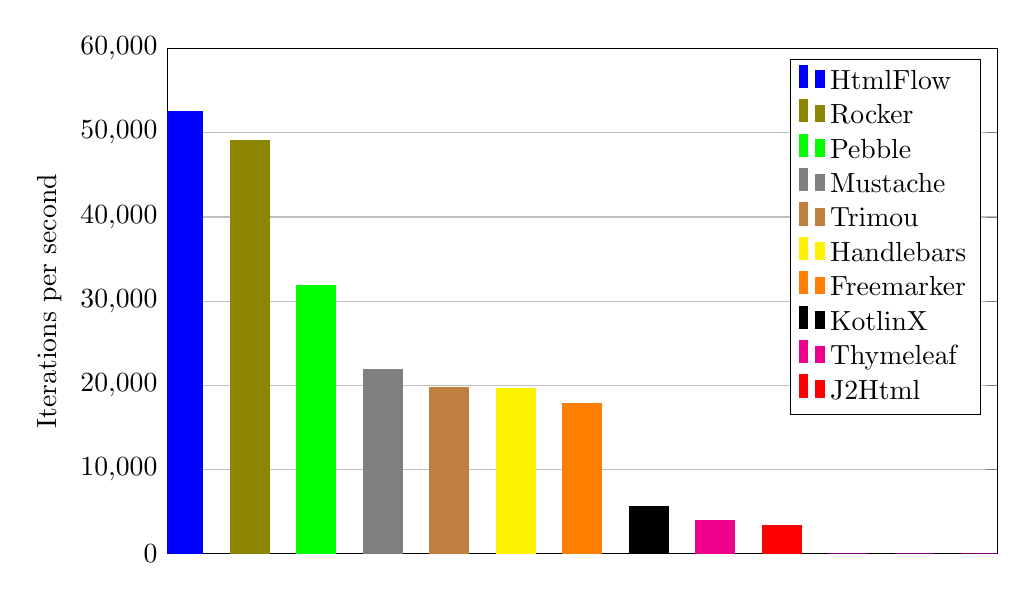
\begin{tikzpicture}
    \begin{axis}[
        width  = 1*\textwidth,
        height = 8cm,
        major x tick style = transparent,
        ybar=1*\pgflinewidth,
        bar width=14pt,
        ymajorgrids = true,
        ylabel = {Iterations per second},
		symbolic x coords={HtmlFlow,Rocker,Pebble,Mustache,Trimou,Handlebars,Freemarker,KotlinX,Thymeleaf,J2Html,dummy1, dummy2, dummy3},
        %xtick = data,
        xticklabels = {},
        scaled y ticks = false,
        enlarge x limits=0.8,
        ymin=0,
        ymax=60000,
        legend cell align=left,]
                
        \addplot[style={blue,fill=blue,mark=none}]
            coordinates {(HtmlFlow, 52463)};
        \addplot[style={olive,fill=olive,mark=none}]
            coordinates {(Rocker, 49107)};
        \addplot[style={green,fill=green,mark=none}]
            coordinates {(Pebble, 31856)};
        \addplot[style={gray,fill=gray,mark=none}]
            coordinates {(Mustache, 21829)};
        \addplot[style={brown,fill=brown,mark=none}]
            coordinates {(Trimou, 19704)};
        \addplot[style={yellow,fill=yellow,mark=none}]
            coordinates {(Handlebars, 19603)};
        \addplot[style={orange,fill=orange,mark=none}]
            coordinates {(Freemarker, 17831)};
        \addplot[style={black,fill=black,mark=none}]
            coordinates {(KotlinX, 5587)};
        \addplot[style={magenta,fill=magenta,mark=none}]
            coordinates {(Thymeleaf, 3965)};
        \addplot[style={red,fill=red,mark=none}]
            coordinates {(J2Html, 3364)};
        \addplot[style={violet,fill=violet,mark=none}]
            coordinates {(dummy1, 0)};
        \addplot[style={violet,fill=violet,mark=none}]
            coordinates {(dummy2, 0)};
        \addplot[style={violet,fill=violet,mark=none}]
            coordinates {(dummy3, 0)};
        \legend{HtmlFlow,Rocker,Pebble,Mustache,Trimou,Handlebars,Freemarker,KotlinX,Thymeleaf,J2Html}
    \end{axis}
\end{tikzpicture}
\caption{Benchmark Stocks - 4 Threads}
\label{fig:benchstocks4threads}
\end{figure}

\noindent
To analyze these results we have to approach two different instances, the more classical \textit{template engines} and the \textit{template engines} that in some way diverge from that classical \textit{template engine} solutions.

\noindent
Regarding the classical \textit{template engines}, i.e. Mustache/Pebble/Freemarker/Trimou/Velocity/Handlebars/Thymeleaf, we can observe that most of them share the same level of performance, which should be expected since they all roughly share the same methodology in their solution. The most notable outlier is Thymeleaf which has a distinct difference to the other \textit{template engines}.

\noindent
Regarding the remaining \textit{template engines}, i.e. Rocker/J2Html/KotlinX, the situation is diverse. On one hand we have Rocker, which presents a great performance when the number of \textit{placeholders} increases, i.e. the Stocks benchmark, taking in consideration that it provides many compile time verifications regarding the context objects it presents a good improvement on the classical template engines solutions. On the other end of the spectrum we have J2Html and KotlinX. Regarding J2Html we observe that the trade off of moving the template to the language had a significant performance cost since it's consistently one of the two worst solutions performance-wise. Regarding KotlinX, the solution that is the most similar to the one that \texttt{xmlet} provides, the results are surprising, since they diverge so much from the results that the HtmlFlow achieves. KotlinX was definitely a step on the right direction since it validates the \ac{HTML} language rules and introduces compile time validations but either due to the Kotlin language performance issues or poorly optimized code it didn't achieve the level of performance that it could achieve.

\noindent
Lastly, the HtmlFlow solution. The use case of the \texttt{xmlet} to the \ac{HTML} language proved to be the best performance wise. The solution achieved values that surpass the second best solution by twice the iterations per second when using the Presentations benchmark and still held the top place in the Stocks benchmark even though the number of \textit{placeholders} for dynamic information increased significantly. If we compare the HtmlFlow to the most similar solution, KotlinX, we observe a huge gain of performance on the HtmlFlow part. The performance improvement varies between HtmlFlow being nine times faster on the Stock benchmark with four threads and thirty one times faster on the Presentations benchmark with four threads. In conclusion the \texttt{xmlet} solution introduces domain language rule verification, removes the requirements of text files and additional syntaxes, adds many compile time verifications and while doing all of that it still is the best solution performance wise.